\documentclass[12pt, twoside]{article}
\usepackage[letterpaper, margin=1in, headsep=0.2in]{geometry}
\setlength{\headheight}{0.6in}
%\usepackage[english]{babel}
\usepackage[utf8]{inputenc}
\usepackage{microtype}
\usepackage{amsmath}
\usepackage{amssymb}
%\usepackage{amsfonts}
\usepackage{siunitx} %units in math. eg 20\milli\meter
\usepackage{yhmath} % for arcs, overparenth command
\usepackage{tikz} %graphics
\usetikzlibrary{quotes, angles}
\usepackage{graphicx} %consider setting \graphicspath{{images/}}
\usepackage{parskip} %no paragraph indent
\usepackage{enumitem}
\usepackage{multicol}
\usepackage{venndiagram}

\usepackage{fancyhdr}
\pagestyle{fancy}
\fancyhf{}
\renewcommand{\headrulewidth}{0pt} % disable the underline of the header
\raggedbottom
\hfuzz=2mm %suppresses overfull box warnings

\usepackage{hyperref}

\fancyhead[LE]{\thepage}
\fancyhead[RO]{\thepage \\ Name: \hspace{4cm} \,\\}
\fancyhead[LO]{BECA / Dr. Huson / Geometry\\*  Unit 1: Segments, length, and area\\* 19 Sept 2022}

\begin{document}

\subsubsection*{1.8 Classwork: Area of rectangles, triangles, parallelograms}
\begin{enumerate}

\item Find the \emph{area} of the shape shown below composed of a rectangle and two semi-circular caps. Leave your answer as an exact value in terms of $\pi$.
\begin{flushright}
\begin{tikzpicture}[scale=.635]
  \draw [help lines] (-1,-1) grid (7,7);
  \draw [thick, ->] (-1.2,0) -- (7.4,0) node [below right] {$x$};
  \draw [thick, ->] (0,-1.2)--(0,7.4) node [left] {$y$};
  \draw [thick] (2,2)--(5,2)--(5,4)--(2,4)--cycle;
  \draw [thick] (2,4) arc (90:270:1);
  \draw [thick] (5,2) arc (-90:90:1);
\end{tikzpicture}
\end{flushright}


\end{enumerate}
\end{document}